\section{Прочие комбинаторные величины}

В этом параграфе мы очень кратко рассмотрим прочие комбинаторные величины, которые могут оказаться полезны и которые будут в дальнейшем выступать в качесве примеров.

\subsection{Числа Фибоначчи}

\begin{definition}
\term{Числа Фибоначчи} $F_n$ определяются начальными условиями $F_0 = 0$, $F_1 = 1$ и соотношением
$$F_{n+1} = F_n + F_{n-1}$$
\end{definition}

Начальные значения чисел Фибоначчи выглядят так:
$$0, 1, 1, 2, 3, 5, 8, 13, 21, 34, 55, \ldots$$

Эти числа возникают в целом ряде задач и довольно распространены. Исторически числа Фибоначчи стали широко известны после решения Леонардо Пизанским (<<Фибоначчи>>  было его прозвищем, что переводится как <<сын Боначчи>>) следующей задачи в 1202 году:

\begin{exercise}
Предположим, что каждая взрослая пара кроликов каждый месяц производит на свет ещё одну молодую пару кроликов. Взросление кроликов наступает в течение одного месяца. Изначально у нас есть одна пара молодых клоликов. Через месяц она становится взрослой. Еще через месяц эта пара производит на свет ещё пару молодых кроликов (итого 2 пары, из которых 1 молодая). В следующий месяц эта же пара производит ещё одну молодую пару, а пара, которая была молодой, взрослеет (имеем 3 пары кроликов, 1 молодая). Таким же образом в следующий месяц мы будем иметь 5 пар кроликов, из которых 2 будут молодыми. Сколько кроликов будет в конце года?
\end{exercise}

На самом деле числа, которые мы сегодня называем числами Фибоначчи, были известны ещё древним Индусам. Математик Пиндас в своём трактате <<Чхандас>> (датированным примерно 200 годом до нашей эры) использует их при решении примерно такой задачи:

\begin{exercise}
Пусть нам надо пройти путь длины $n$. При проходе пути мы можем использовать либо шаги длины 1, либо шаги длины 2. Докажите, что существует ровно $F_{n+1}$ способов пройти путь используя такие шаги. (Например для пути длины 3 мы можем сделать три одинарных шага, либо вначале одинарный, а потом двойноё, либо наоборот: итого 3 разных способа пройти путь).
\end{exercise}

Сами индусы, правда, решали хоть и ту же задачу, но из другой предметной области: они исследовали сколько всего существует мелодий, состоящих лишь из одной ноты, которая может иметь либо одинарную, либо двойную длительность. Интерпретация, данная привёденным мной упражнением, используется при решении следующих двух задач:

\begin{exercise}
Докажите следующее тождество, используя двойной счёт:
$$F_{n+1} = \sum_{k=0}^{\lfloor {n\over 2}\rfloor} {n-k\choose k}$$
\end{exercise}

\begin{exercise}
Докажите следующее тождество (идея доказательства очень похожа):
$$F_{n+1} = 1+ \sum_{k=0}^{n-1}F_n$$
\end{exercise}

\begin{thm}
$$F_n F_{n+1} = \sum_{i=1}^n F_i^2$$
\end{thm}
\begin{figure}[h]
\centering
\begin{tikzpicture}
\draw (0, 0) rectangle (6.5cm, -4cm);
\draw (2.5cm, 0) -- (2.5cm, -4cm);
\draw (0, -1.5cm) -- (2.5cm, -1.5cm);
\draw (1cm, 0) -- (1cm, -1.5cm);
\draw (0, -.5cm) -- (1cm, -.5cm);
\draw (.5cm, 0) -- (.5cm, -.5cm);
\end{tikzpicture}
\caption{Прямоугольник Фибоначчи}
\end{figure}
\begin{proof}
Идея докательства продемонстрирована на рисунке~3.13. Прямоугльник Фибоначчи строится следующим образом: вначале рисуем квадрат единичной длиной стороны. Затем справа от него рисуем ещё один такой же квадрат. После под ними рисуем квадрат со стороной равной двум предыдущим квадратам. Затем справа рисуем опять квадрат со стороной, равной двум предыдущим. Совершая последовательно $n$ таких построений, в итоге имеем прямоугольник со сторонами $F_n$ и $F_{n+1}$. Всего его площадь (то есть количество единичных квадратиков, которые в него уместятся), равно $F_nF_{n+1}$. В то же время подсчитав площади квадртав в порядке построения получаем сумму  $\sum_{i=1}^n F_i^2$.
\end{proof}

Следующая наша теорема (называемая теоремой Цекендорфа) утверждает, что любое натуральное число можно представить единственным образом в виде суммы чисел Фибоначчи таким образом, что каждое из чисел будет использоваться максимум единожды, и что в этой сумме не будет присутствовать никакие два последовательные числа Фибоначчи. Числа $F_1$ и $F_0$ в этом представлении так же не учавтсвуют. Таким образом, для любого $a$ мы можем записать:
\begin{equation}\label{non:1}
a = \sum_{i=1}^m F_{\alpha_i}
\end{equation}
где $\alpha_k$~--- это последовательность номеров использованных чисел Фибоначчи.

Помимо интересного практического применения этой теоремы (о чём я напишу несколькими абзацами ниже), такое представление позволяет определить операцию <<Фибоначчиевого умножения>>. Пусть, например, мы представили число $b$ так же в соответствии с теоремой Цекендорфа:
$$b = \sum_{j=1}^n F_{\beta_j}$$

Тогда множение Фибоначчи определяется таким образом:
$$a\circ b = \sum_{i=1}^m\sum_{j=1}^n F_{\alpha_i+\beta_j}$$

\begin{exercise}
Покажите, что $2\circ3 = 13$ и что $4\circ4 = 40$.
\end{exercise}

Легко видеть, что такое умножение коммутативно ($a\circ b = b\circ a$), однако довольно неожиданно, что оно так же является и ассоциативным, то есть выполняется тождество
$$a\circ(b\circ c) = (a\circ b)\circ c$$

Это в общем-то единственное полезное свойство такого умножения, но сам факт довольно интересен и неожиданнен. Доказательство, которое я представляю ниже, сделает это утверждение очевидным.

\begin{thm}
Любое число $n$ допускает единственное представление в виде \eqref{non:1}.
\end{thm}
\begin{proof}
Данная теорема может быть легко доказана по индукции (что и сделал в 1972 году Цекендорф), однако я представлю более остроумное доказательство, придуманное Дональном Кнутом в 1988 году. В той же работе Кнут ввёл понятие Фибоначчиева умножения и показал его ассоциативность, как простое следствие из данное доказательства.

Теорему Цекендорфа можно переформулировать как возможность представить любое число в виде суммы
$$\sum_{i=0}^n d_iF_i$$
где коэффициенты $d_i$ могут принимать значения 0 или 1, причем два коэффициента подряд не могут принимать значение 1. Такую запись называют <<системой счисления Фибоначчи>>, поскольку она очень похожа на позиционные системы счисления, рассмотренные нами в~\S3.2, с той лишь разницей, что теперь вместо степеней некоторого основания мы используем значения $F_i$. По аналогии с позиционными системами счисления мы можем кратко записывать числа в ней, перечисляя последовательно коэффициенты $d_i$. Чтобы отличать Фибоначчиеву систему счисления, мы будем подписывать букву $f$ справа от записи. Например,
$$33 = 101010100_f$$
Два младных разряда (соответствующие $F_0$ и $F_1$) всегда равны нулю.

Чтобы получить такую запись, мы вначале позволим коэфициентам $d_i$ принимать произвольные значения, а затем путём их преобразований будем пошагово идти к требуемому представлению. Заметим, что при отсутствии ограничений на коэффициенты, представить натуральное число $a$ в виде суммы чисел Фибоначчи не представляет труда: достаточно взять значения $d_2 = a$ и $d_i = 0$ в остальных случаях (или, иначе, можно применить тот же подход с остатками от деления, который мы применяли при построении позиционных систем счисления).

Пусть мы получили некоторую запись натурального числа и в ней имеется коэффициент $d_i > 1$. Здесь может быть две ситуации: когда $d_{i-1}> 0$ и когда $d_{i-1} = 0$. В первом случае мы можем увеличить на единицу значение $d_{i+1}$ и уменьшить на единицу значения $d_i$ и $d_{i-1}$ по определнию чисел Фибоначчи. Зачему, что то же преобразование мы можем выполнить в случае
$$d_i = d_{i-1} = 1$$
Если же $d_{i-1} = 0$, то мы можем уменьшить на единицу $d_i$ и увеличить на единицу $d_{i-1}$ и $d_{i-2}$. Мы пришли к ситуации, когда $d_{i-1} > 0$, а как действовать в этом случае мы уже знаем. Применив указанное выше преобразование мы получаем суммарно, что мы увеличили на единицу $d_{i+1}$, уменьшили на двойку $d_i$ и на единицу $d_{i-2}$.

Если в ходе эти преобразований мы на каком-то шаге получаем $d_0 > 0$, то это можно безболезненно заменять на $d_0 = 0$. Если мы получили $d_1 > 0$, то можно смело прибавлять величину $d_1$ к $d_2$ зануляя $d_1$.

Здесь важно заметить два момента: во-первых, если рассматривать набор коэффициентов $\{d_i\}$ как упорядоченный набор, то после каждого такого преобразования новый набор будет больше старого в смысле лексикографического порядка. Применять одно из указанных преобразований мы можем всегда, если только наше число не представлено уже в требуемом виде. В то же время само множество допустимых наборов у нас ограничено, поскольку всегда найдётся $F_n > a$, так что продолжать применять бесконечно долго наши правила преобразования мы не сможем. Таким образом в итоге мы обязательно придём к Фибоначчиевому представлению числа.

Из этой интерпретации легко увидеть и единственность такого представления. Если нам даны два различных таких представления то мы можем вычесть большее в лексикографическом смысле из меньшего. Здесь правда может возникнуть проблема, что нам придётся вычитать единицу из нуля. Будем писать в этом случае $d_i =-1$, что означает, что этого слагаемого нам недостаёт. Поскольку мы вычитаем большее из меньшего, всегда найдётся такое $k$, что $d_{i+k} = 1$. Его можно занулить, увеличив на единицу значения $d_{i+k - 1}$ и $d_{i+k-2}$. Повторяя эту операцию несколько раз мы можем избавиться от всех значений $-1$, однако результат будет ненулевым, т.к. каждая такая операция не может уменьшать количество единиц в записи. Значит, рахзница между двумя представлениями положительно, а следовательно эти представления всё же задают различные числа.
\end{proof}

Очевидно теперь, что фибоначчиево умножение~--- это просто умножение чисел в столбик, с тем только лишь отличием, что мы на этот раз используем фибоначчиеву систему счисления. Отсюда уже легко понять, почему оно ассоциативно (поймите это в качестве упражнения).

Рассмотрим задачу передачи данных по сети. Для просторы будем считать, что мы последовательно передаём числа в диапазоне от 0 до 15 (на практике мы бы вероятнее всего были заинтересоаны в передаче полноценных байтов в диапазоне от 0 до 255). Кодировать числа мы будем битами 1 и 0, что означает наличие и отсутствие напряжения соответственно. Мы легко можем передать значения, используя простое двоичное представления. Пусть, например, мы хотим передать числа 11, 13 и 10. В двоичной записи мы передадим следующие данные:
$$1011\ 1101\ 1010\ \ldots \cong 11,13,10,\ldots$$
Однако, при передаче по сети данные могут теряться из-за помех. Пусть, например, мы потеряли четвёртый бит. Тогда полученные данные будут выглядеть как
$$1011\ 1011\ 0100\ \cong 11, 11, 4, \ldots$$
Очевидно, что все последние данные так же будут повреждены и получатель данных в результате получит совершенно бессмысленый набор данных. Если, например, эти данные~--- это видеотрансляция, то пропажа всего одного бита в потоке (что очень вероятно) по сути приведёт к неутранимой ошибке, что заставит пользователя устанавливать соединение заново. Это явно неприемлемо.

Фибоначчиева система счисления может решить проблему. Её критическим свойством является то, что в ней не могут идти подряд два бита 1, а значит мы можем использовать битовую последовательность 11 для разделения фрагментов данных. Для экономии трафика мы можем немного сэкономить место, избавившись, во-первых, от разрядов $d_0$ и $d_1$ (они всегда нулевые), а так же передавая запись в обратном порядке. Это гарантирует нам, что старшим битом в записи всегда будет 1, поэтому мы можем дописывать всего один бит 1 к нему, а не биты 11. Например, если закодировать таким образом $11=1010000_f$, то в итоге получим значение $001011$, что короче на один бит. Данные, приведённые выше, будет таким образом переданы в виде
$$001011\ 0000011\ 010011\ \ldots \cong 11, 13, 10, \ldots$$
Если теперь у нас произойдёт ошибка связи и какой-то бит потеряется, вставится или изменится, мы конечно получим какие-то данные в ошибочном виде, однако мы всегда знаем, что новое значение начинается после последовательности 11, поэтому любое повреждение будет иметь лишь локальный смысл. Опять же в случае видеопотока такое повреждение будет означать, что мы будем иметь помеху в нескольких каждрах, однако эта помеха сама же и устранится, т.к. последующие данные мы будем получать уже в корректном виде.

На практике, впрочем, разработано множество других более совершенных систем кодирования, но их мы касаться не будем.

\subsection{Числа Каталана}

\begin{definition}
\term{Числа Каталана} $C_n$ определяются начальным значением $C_0 = 1$ и условием
$$C_{n+1} = \sum_{k=0}^n C_kC_{n-k}$$
\end{definition}

Начальные значения чисел Каталана выглядят так:
$$1, 1, 2, 5, 14, 42, 132, 429, 1430, 4862, 16796, \ldots$$

Как и числа Фибоначчи, они возникают во многих задачах. Рассмотрим, например, количество строк длин $n$, состоящих из парных скобок (то есть строк типа "((()()))(())"). Пусть у нас имеется $n+1$ парная скобка. Возьмём первую пару (то есть скобки "(...)..."). Предположим, что внутри этой пары находится $k$ пар скобок. Тогда после этой пары скобок будет находиться ещё $n-k$ пар скобок. По индукции это даёт нам, что всего таких строк есть $C_kC_{n-k}$ штук. Суммируя теперь по всем значениям $k$ получаем, что количество таких строк определяется числами Каталана.

Давайте теперь подсчитаем количество спобов вычислить сумму (или любую другую ассоциативную операцию) $n+1$ слагаемых. В силу ассоциативности количество вычислить эту сумму равно количеству способов расставить $n$ пар скобок в этой записи. Итого опять же получаем, что это количество спобов равно величине $C_n$.

По расстановке скобок в сумме мы можем построить бинарное дерево. Пусть у нас есть $n+1$ слагаемое. Вначале сопоставим каждому слагаемому в соответствие узел дерева (эти узлы будем называть \term{внешними}~--- они не будут имеют потомков). Затем каждой арифметической операции будем ставить в соответствие узел дерева с двумя потомками, соответствующими складываемым значениям (будем называть такие узлы \term{внутренними}). Очевидно, что такие деревья однозначно соответствуют расстановкам скобок, а следовательно таких деревьев будет $C_n$ штук. Здесь $n$~--- это количество операций, оно же количество внутренних узлов (внешних соответствунно $n+1$). Если отбросить интерпретацию со слагаемыми, внешними и внутренними узлами, то получаем, что всего бинарных деревьев с $n$ узлами имеется $C_n$ штук. Рисунок~3.14 демонстрирует идею.

\begin{figure}[h]
\centering
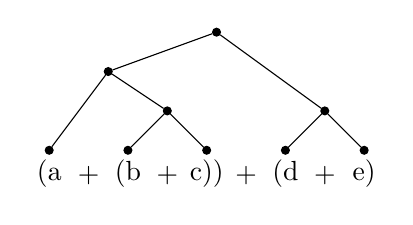
\begin{tikzpicture}
\def\point{node [circle, draw, fill, inner sep = 0, minimum size = .1cm] }
\def\emptynode{node [draw=none,fill=none, below] }
\draw (-2cm, 0) \point (p1) {};
\draw (-1.5cm, .05cm) \emptynode (s12) {};
\draw (-1cm, 0) \point (p2) {};
\draw (-.5cm, .05cm) \emptynode (s23) {};
\draw (0cm, 0) \point (p3) {};
\draw (.5cm, .05cm) \emptynode (s34) {};
\draw (1cm, 0) \point (p4) {};
\draw (1.5cm, .05cm) \emptynode (s45) {};
\draw (2cm, 0) \point (p5) {};

\draw (-.5cm, .5cm) \point (p23) {};
\draw (1.5cm, .5cm) \point (p45) {};
\draw (-1.25cm, 1cm) \point (p123) {};
\draw (.125cm, 1.5cm) \point (p12345) {};

\node [below] at (p1) {(a};
\node [below] at (s12) {+};
\node [below] at (p2) {(b};
\node [below] at (s23) {+};
\node [below] at (p3) {c))};
\node [below] at (s34) {+};
\node [below] at (p4) {(d};
\node [below] at (s45) {+};
\node [below] at (p5) {e)};

\draw (p23) -- (p2);
\draw (p23) -- (p3);
\draw (p45) -- (p4);
\draw (p45) -- (p5);
\draw (p123) -- (p1);
\draw (p123) -- (p23);
\draw (p12345) -- (p123);
\draw (p12345) -- (p45);
\end{tikzpicture}
\caption{Бинарное дерево, построенное по выражению.}
\end{figure}

Стоит отдельно заострить внимание на отличиях от тех деревьев, формулу для числа которых мы получили в теореме~3.42:
\begin{enumerate}
\item Дерево обладает корнем;
\item Вершины не имеют именований, важна только их форма;
\item Каждая вершина может иметь максимум двух потомков;
\item Рёбра упорядочены, то есть важно, нарисовано оно слева или справа от узла.
\end{enumerate}

На самом деле та же величина за небольшой оговоркой показывает и количество произвольных деревьев. Для того, чтобы увидеть это, нам потребуется следующее определение.

\begin{definition}
\term{Лесом} называется граф, состоящий из нескольких несвязанных деревьев.
\end{definition}

Опять же леса рассматриваются в математики разные, но нас будут интересовать лишь те, в которых упорядочены как сами деревья, так и их рёбра. Оказывается, что между бинарными деревьями и лесами можно построить взаимооднозначное соответствие. Я покажу как по лесу построить бинарное дерево, процедура в обратную сторону совершенно аналогична.

В качестве корня бинарного дерева выбирается корень первого дерева в лесе. На рисунке 3.15 это узел $a$. Затем по левой ветви мы строим опять же бинарное дерево, которое строится по аналогии, если рассматривать первое дерево за вычетом корня, как лес (в примере на рисунке это лес, состоящий из деревьев d-h, e-i и f). По правой ветви мы строим бинарное дерево для леса, получающегося после удаления первого дерева (в примере это лес, состоящий из деревьев b-g и c).

\begin{figure}[h]
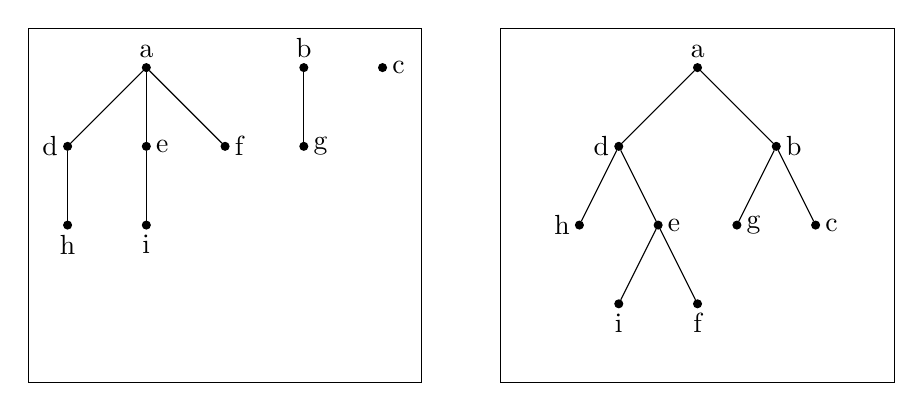
\begin{tikzpicture}
\def\point{node [circle, draw, fill, inner sep = 0, minimum size = .1cm] }
\draw (-1cm, 0) \point (lc) {};
\draw (-2cm, 0) \point (lb) {};
\draw (-2cm, -1cm) \point (lg) {};
\draw (-4cm, 0) \point (la) {};
\draw (-4cm, -1cm) \point (le) {};
\draw (-5cm, -1cm) \point (ld) {};
\draw (-3cm, -1cm) \point (lf) {};
\draw (-5cm, -2cm) \point (lh) {};
\draw (-4cm, -2cm) \point (li) {};

\node [right] at (lc) {c};
\node [above] at (lb) {b};
\node [right] at (lg) {g};
\node [above] at (la) {a};
\node [left] at (ld) {d};
\node [right] at (le) {e};
\node [right] at (lf) {f};
\node [below] at (lh) {h};
\node [below] at (li) {i};

\draw (lb) -- (lg);
\draw (la) -- (ld);
\draw (ld) -- (lh);
\draw (la) -- (le);
\draw (le) -- (li);
\draw (la) -- (lf);

\draw (-5.5cm, .5cm) rectangle (-.5cm, -4cm);


\draw (3cm, 0) \point (ra) {};
\draw (2cm, -1cm) \point (rd) {};
\draw (4cm, -1cm) \point (rb) {};
\draw (1.5cm, -2cm) \point (rh) {};
\draw (2.5cm, -2cm) \point (re) {};
\draw (3.5cm, -2cm) \point (rg) {};
\draw (4.5cm, -2cm) \point (rc) {};
\draw (2cm, -3cm) \point (ri) {};
\draw (3cm, -3cm) \point (rf) {};

\node [above] at (ra) {a};
\node [right] at (rb) {b};
\node [right] at (rc) {c};
\node [left] at (rd) {d};
\node [right] at (re) {e};
\node [below] at (rf) {f};
\node [right] at (rg) {g};
\node [left] at (rh) {h};
\node [below] at (ri) {i};

\draw (ra) -- (rd);
\draw (rd) -- (rh);
\draw (rd) -- (re);
\draw (re) -- (ri);
\draw (re) -- (rf);
\draw (ra) -- (rb);
\draw (rb) -- (rg);
\draw (rb) -- (rc);

\draw (5.5cm, .5cm) rectangle (.5cm, -4cm);
\end{tikzpicture}
\caption{Соответствие леса и бинарного дерева.}
\end{figure}

Теперь мы готовы к тому, чтобы понять сколько всего произвольных деревьев с $n$ вершинами существует. Если применить соответствие лес-бинарное дерево, то бинарное дерево, полученное из произвольного дерева, не будет иметь правой ветви у корня, левое же поддерево может быть произвольным бинарным. Итого у нас есть свобода выбора как расположить в дереве $n-1$ узел. Итого произвольных деревьев $n$ вершинами существует $C_{n-1}$ штук.

Ну и так далее. Числа Каталана всплывают постоянно и мне даже кажется довольно странным, что они довольно мало известны в народе, в отличие от тех же чисел Фибоначчи, которые применяют даже биржевые трейдеры (последние верят, что числа Фибоначчи имеют какое-то психологически-сакральное значение, что позволяет им предсказывать поведение цен на рынке). Думаю, в пользе чисел Каталана я вас убедил. Остаётся вопрос как можно их более эффективно находить.

Числа Каталана можно интерпретировать ещё вот как. Рассмотрим квадрат размером $n\times n$. Координаны в этом квадрате будем записывать парой $(x, y)$, которую будем называть \term{координатами}, и в которой $x$ и $y$ могут принимать значения от 0 до $n$. Мы начинаем движение из точки с координатами $(0, 0)$ и двигаемся в точку $(n, n)$, увеличивая за один шаг на единицу либо координату $x$, либо координату $y$. Числа Каталана в этом случае показывают количество путей, которые не пересекают диагональ квадрата (то есть никогда не заходят в точку с координатами $(x, x+1)$).

Увидеть это довольно легко по индукции. Пусть утверждение уже доказано для квадратов размером вплоть до $n$ и мы рассматриваем количество путей в квадрате со сторонами $n+1$. Пусть при движении мы в последний касаемся диагонали в позиции $(k, k)$. Количество способов пройти такой путь до точки касания есть $C_k$ (по предположению индукции). После этого дойти до финиша не коснувшись диагонали у нас остаётся $С_{n-k}$ способов (пройти нам надо ещё $n-k+1$ клетку, однако учитывая, что мы не должны касаться диагонали, первый шаг у нас увеличит координату $x$, а последний координату $y$, что по сути сводит задачу к нахождению пути в квадрате со стороной $n-k$). Отсюда следует, что такие пути так же задаются числами Каталана.

С другой стороны те читатели которые читают учебник последовательно, помнят, что вообще-то ровно то же самое количество путей не пересекающих диагональ квадрата предлагалось найти в упражнении~3.60 используя только понятие сочетаний. Я покажу сейчас как решается та задача.

Вначале поймём сколько вообще существует путей, увеличивающих за шаг лишь одну координату, без учёта пересечения диагонали (упражнение~3.59). Если размеры прямоугольинка $m\times n$, то нам надо $m$ раз увеличить координату $x$ и $n$ раз координату $y$. Итого нам надо совершить $m+n$ шагов, из которых надо выбрать $m$ шагов, которые увеличивают $x$. Способов сделать такой выбор имеется ${m + n \choose m}$. В случае, если нам дан квадрат размером $n\times n$, то очевидно количество путей будет равно ${2n\choose n}$.

\begin{figure}[h]
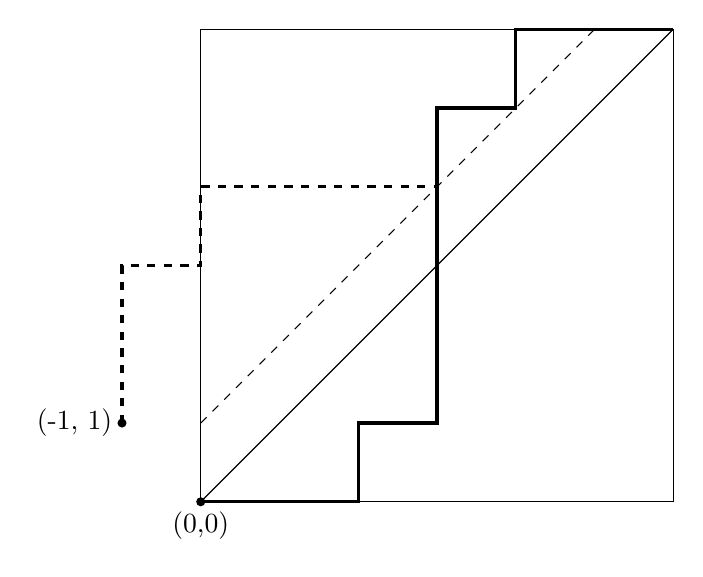
\begin{tikzpicture}
\def\point{node [circle, draw, fill, inner sep = 0, minimum size = .1cm] }
\centering
\draw (-3cm, -3cm) rectangle (3cm, 3cm);
\draw (-3cm, -3cm) \point (z) {};
\node [below] at (z) {(0,0)};

\draw (-3cm, -3cm) -- (3cm, 3cm);

\draw [very thick] (-3cm, -3cm) -- (-1cm, -3cm) -- (-1cm, -2cm) -- (0, -2cm) -- (0, 2cm) -- (1cm, 2cm) -- (1cm, 3cm) -- (3cm, 3cm);
\draw [dashed] (-3cm, -2cm) -- (2cm, 3cm);
\draw [very thick, dashed] (-4cm, -2cm) -- (-4cm, 0) -- (-3cm, 0) -- (-3cm, 1cm) -- (0, 1cm);

\draw (-4cm, -2cm) \point (t) {};
\node [left] at (t) {(-1, 1)};

\end{tikzpicture}
\caption{Отражение начала пути от диагонали.}
\end{figure}

Рассмотрим теперь путь, который диагональ всё же пересекает. Пусть первое пересечение происходит в позиции $(k, k+1)$. Давайте отразим часть пути до этой точки относительно диагонали, сдвинутой вверх на единицу (см. рисунок 3.16). При этом получится некий путь, начинающийся в координатах $(-1, 1)$ и идущий в точку $(n, n)$. Таких путей ровно ${2n\choose n-1}$ штук, поскольку они описывают движение в прямоугольнике $((n-1)\times (n+1)$. Легко так же увидеть, что все пути из точки $(-1, 1)$ после отражения их от начала до точки пересечения диагонали (а они её пересекут обязательно) дают нам путь, который нас не устраивает. Итого нам осталось вычесть количество <<неправильных путей>> из общего числа путей:
$$C_n = {2n\choose n} - {2n\choose n-1} = {{2n\choose n}\over n+1}$$
Последнее равенство легко проверяется, я предлагаю выполнить вам проверку в качестве упражнения.